\documentclass[11pt,a4paper]{article}
\usepackage[margin=2.5cm]{geometry}
\usepackage{amsmath,amssymb,booktabs,array,enumitem,xcolor,parskip,graphicx,float,caption,tabularx,listings,adjustbox}
\usepackage[colorlinks=true,urlcolor=blue,linkcolor=black]{hyperref}

\newcommand{\ok}[1]{\textcolor{green!40!black}{#1}}
\newcommand{\bad}[1]{\textcolor{red!70!black}{#1}}
\newcommand{\jawab}[1]{\subsection*{#1}\addcontentsline{toc}{subsection}{#1}}
\newcommand{\fig}[3]{\begin{figure}[H]\centering\includegraphics[width=#2\textwidth]{figures/#1}\caption{#3}\end{figure}}
\newcolumntype{L}{>{\raggedright\arraybackslash}X}
\setlist{itemsep=2pt,topsep=2pt}
\captionsetup{font=small,labelfont=bf}
\renewcommand{\contentsname}{Daftar Isi}
\renewcommand{\figurename}{Gambar}
\renewcommand{\tablename}{Tabel}

\lstset{basicstyle=\ttfamily\footnotesize,breaklines=true,frame=single,columns=fullflexible,
        keywordstyle=\color{blue!60!black}\bfseries,commentstyle=\color{green!40!black},
        stringstyle=\color{red!50!black},language=Python,showstringspaces=false}

\title{Laporan Ujian Tengah Semester\\[2pt]\large Kecerdasan Buatan (TE2514031), Semester Gasal 2026/2027\\[2pt]
\normalsize Soal 3 (GA), Soal 7 (PSO), Soal 12 (Fuzzy Logic), Soal 16 (Neural Network), Soal 23 (PSO-CNN)}
\author{Marsa Naufal (04231047)}
\date{27 Oktober 2026}

\setlength{\emergencystretch}{3em}
\begin{document}
\maketitle
\tableofcontents
\newpage

\section{Pendahuluan}

Saya mendapat lima soal UTS, satu dari setiap kelompok: Genetic Algorithm (Soal 3), Particle Swarm Optimization (Soal 7), Fuzzy Logic (Soal 12), Neural Network (Soal 16), dan algoritma gabungan (Soal 23). Semuanya saya kerjakan di Python, satu notebook Jupyter per soal, dan setiap notebook bisa dijalankan ulang. Angka dan grafik di laporan ini diambil langsung dari output notebook tersebut.

\subsection*{Pengaturan umum}
\begin{tabularx}{\textwidth}{@{}lL@{}}
\toprule
\textbf{Hal} & \textbf{Keterangan} \\
\midrule
Seed & 47 (dua digit terakhir NIM 04231047), dipakai untuk semua proses acak: split data, inisialisasi GA/PSO, dan bobot neural network. \\
Bahasa \& library & Python 3.13; \texttt{pygad} (GA), \texttt{pyswarms} (PSO), \texttt{scikit-fuzzy} (Mamdani FIS), \texttt{PyTorch} (MLP dan 1D-CNN), \texttt{scikit-learn}, \texttt{pandas}, \texttt{numpy}, \texttt{scipy}, \texttt{matplotlib}. \\
Dataset & UCI: D4 Wine Quality (red), D3 Energy Efficiency, D6 Electrical Grid Stability, D8 Auto MPG, D9 Human Activity Recognition. \\
Aturan test set & Test set tidak pernah dipakai untuk memilih hyperparameter, threshold, versi rule, maupun membership function. Semua pemilihan memakai data latih atau validation. \\
Notebook & \texttt{soal\_03\_ga.ipynb}, \texttt{soal\_07\_pso.ipynb}, \texttt{soal\_12\_fuzzy.ipynb}, \texttt{soal\_16\_mlp.ipynb}, \texttt{soal\_23\_pso\_cnn.ipynb} \\
\bottomrule
\end{tabularx}

\subsection*{Alur pengerjaan}
Setiap soal saya kerjakan mengikuti tahapan sains data. Bagian Business Understanding berisi latar belakang dan kriteria kesuksesan yang ambangnya saya tetapkan sebelum eksperimen. Data Understanding memeriksa sampel, atribut, statistik, missing value, duplikasi, dan outlier, lalu Data Preparation menjelaskan pembersihan, split, encoding, dan scaling beserta alasannya. Modeling dan Evaluation memuat jawaban butir (a) sampai (d). Interpretasi Hasil menguji model pada data yang belum pernah dilihat dan mengecek kriteria kesuksesan.

Bagian Data Understanding di laporan ini saya ringkas. Sampel 20 baris dan tabel statistik lengkapnya ada di notebook masing-masing.

\newpage
\section{Soal 3: Seleksi Fitur Fisikokimia Wine dengan Genetic Algorithm}

Dataset yang dipakai adalah D4 Wine Quality (red wine) dengan 1.599 sampel dan 11 fitur fisikokimia. GA dijalankan dengan \texttt{pygad}.

\subsection{Business Understanding}
Produsen wine ingin tahu kandungan kimia apa yang paling membedakan wine berkualitas tinggi dari yang rendah, supaya uji laboratorium cukup difokuskan ke beberapa parameter. Mirip dokter yang memeriksa beberapa tanda vital yang paling informatif, tidak semua organ.

Ada tiga hal yang ingin dijawab: subset fitur mana yang memaksimalkan skor $J(S)$, apakah GA memberi jawaban yang sama di seed berbeda, dan apakah fitur yang terpilih memang punya distribusi berbeda antar-kelompok. Kriteria kesuksesannya saya tetapkan sebelum eksperimen:

\begin{tabularx}{\textwidth}{@{}LL@{}}
\toprule
\textbf{Kriteria kesuksesan} & \textbf{Ambang} \\
\midrule
GA mencapai optimum hasil \emph{brute force} ($2^{11} = 2048$ subset) & selisih $J$ = 0 \\
Konsistensi antar-run (5 seed) & $\geq$ 4 dari 5 run menghasilkan subset sama \\
Fitur terpilih berbeda signifikan antar-kelompok & Mann-Whitney $p < 0.05$ \\
Subset tetap memisahkan kelas di data \emph{hold-out} & balanced accuracy $\geq 0.75$ \\
\bottomrule
\end{tabularx}

\subsection{Data Understanding dan Data Preparation}
Datanya tidak punya missing value, tetapi ada 240 baris duplikat (sekitar 15\%). Outlier paling banyak muncul di \textit{residual sugar} (155) dan \textit{chlorides} (112), dan keduanya miring ke kanan. Skor \textit{quality} menumpuk di 5 dan 6. Dari korelasi, \textit{alcohol} paling berhubungan positif dengan kualitas dan \textit{volatile acidity} paling negatif.

Duplikat saya buang, karena baris kembar terhitung dua kali di mean dan std, dan salinannya bisa jatuh ke data latih dan \emph{hold-out} sekaligus. Sesuai soal, kelompok H berisi $q \geq 7$, kelompok L berisi $q \leq 5$, dan $q = 6$ dibuang. Outlier tetap dipakai karena merupakan hasil uji lab yang sah. Setelah itu tersisa 824 sampel (H = 184, L = 640).

Data lalu dibagi 80:20 secara berstrata. $J(S)$ dan GA hanya melihat data latih (659 sampel), sedangkan 165 sampel \emph{hold-out} baru dipakai di akhir untuk memeriksa apakah subset terpilih memang informatif. Scaling tidak diperlukan, karena $J(S)$ sudah membagi selisih mean dengan simpangan baku sehingga satuannya hilang.

\fig{soal_03_1.png}{0.9}{Distribusi skor \textit{quality} dan korelasi tiap fitur dengan \textit{quality}.}

\jawab{Jawaban 3a: Makna komponen $J(S)$, penalti, dan kromosom kosong}
\[ J(S) = \sum_{j \in S} \frac{|\mu_{H,j} - \mu_{L,j}|}{\sigma_{H,j} + \sigma_{L,j} + \varepsilon} - 0.10\,|S| \]

\begin{tabularx}{\textwidth}{@{}lL@{}}
\toprule
\textbf{Komponen} & \textbf{Makna} \\
\midrule
$|\mu_{H,j} - \mu_{L,j}|$ & Jarak rata-rata fitur $j$ antara wine bagus dan wine jelek. Makin jauh, makin membedakan. \\
$\sigma_{H,j} + \sigma_{L,j}$ & Sebaran nilai di tiap kelompok. Selisih rata-rata 1 tidak berarti apa-apa kalau data menyebar $\pm$10, tetapi sangat berarti kalau sebarannya hanya $\pm$0.1. Pembagian ini membuat skor tanpa satuan, mirip \emph{signal-to-noise ratio}. \\
$\varepsilon$ & Angka sangat kecil ($10^{-9}$) supaya tidak terjadi pembagian dengan nol. \\
$-0.10|S|$ & Penalti 0.10 untuk setiap fitur yang dipakai. \\
\bottomrule
\end{tabularx}

Penalti diperlukan karena setiap suku pemisahan bernilai $\geq 0$. Tanpa penalti, menambah fitur tidak pernah menurunkan $J$, sehingga jawaban terbaik selalu ``pakai semua fitur''. Dengan penalti 0.10, sebuah fitur harus membayar semacam tiket masuk: ia hanya layak dipakai kalau skor pemisahannya lebih dari 0.10.

Kromosom kosong (semua gen 0) secara rumus menghasilkan $J = 0$, padahal tanpa fitur tidak ada yang bisa dipisahkan. Saya memberinya fitness $-10$. Subset valid tidak mungkin bernilai di bawah $-0.10 \times 11 = -1.1$ karena skor pemisahan selalu $\geq 0$, jadi kromosom kosong selalu kalah dan cepat hilang dari populasi.

Satu hal yang membantu pemeriksaan: $J(S)$ adalah jumlah skor per fitur, dan fitur-fitur itu tidak saling mempengaruhi. Optimum sebenarnya bisa dicari dengan mencoba semua 2048 subset, dan hasilnya ($J = 2.4708$ dengan 8 fitur) saya pakai sebagai kunci jawaban untuk menilai GA.

\jawab{Jawaban 3b: Desain GA dan pengaruh \emph{mutation rate}}
\begin{tabularx}{\textwidth}{@{}llL@{}}
\toprule
\textbf{Komponen} & \textbf{Pilihan} & \textbf{Alasan} \\
\midrule
Representasi & biner, 11 gen & satu gen = saklar satu fitur \\
Populasi / generasi & 30 / 50 & ruang solusi hanya 2048, jadi 30 individu sudah beragam \\
Jumlah orang tua & 10 per generasi & sepertiga populasi, cukup beragam tanpa memberi kesempatan pada individu lemah \\
Seleksi & \emph{tournament}, $k = 3$ & tekanan seleksi sedang, populasi tidak terlalu cepat seragam \\
Crossover & \emph{uniform}, $p = 0.9$ & urutan fitur tidak bermakna, jadi tiap gen diwarisi acak \\
Mutasi & \emph{random} pada \{0,1\}, $p = 0.10$ & peluang gen benar-benar terbalik sekitar 0.05 \\
Elitisme & 2 individu & solusi terbaik tidak pernah hilang \\
\bottomrule
\end{tabularx}

Mutasi bisa dibayangkan sebagai rasa penasaran populasi. Untuk melihat pengaruhnya, GA saya jalankan dengan lima nilai \emph{mutation rate}, masing-masing dengan 5 seed:

\begin{adjustbox}{max width=\textwidth}\begin{tabular}{@{}lcccc@{}}
\toprule
\textbf{Mutation rate} & \textbf{Run capai optimum} & \textbf{Rata-rata generasi capai} & \textbf{Mean fitness akhir} & \textbf{Keragaman akhir} \\
\midrule
0.01 & 5/5 & 5.2 & 2.438 & 0.33 \\
0.05 & 5/5 & 4.4 & 2.335 & 1.23 \\
0.10 & 5/5 & 4.4 & 2.135 & 3.04 \\
0.30 & 5/5 & 8.2 & 1.597 & 5.15 \\
0.60 & \bad{2/5} & 6.5 & 1.204 & 5.52 \\
\bottomrule
\end{tabular}\end{adjustbox}

Dengan 0.01, keragaman akhir tinggal 0.33 bit, artinya hampir semua individu sudah kembar dan populasi rawan konvergensi prematur. Di soal ini hasilnya masih aman hanya karena ruang solusinya kecil. Nilai 0.05 sampai 0.10 menemukan optimum paling cepat (rata-rata generasi ke-4,4) sambil tetap menjaga populasi beragam, jadi 0.10 saya pakai untuk GA utama. Di 0.60, GA hampir berubah menjadi \emph{random search} dan hanya 2 dari 5 run yang sampai ke optimum.

\jawab{Jawaban 3c: Hasil 5 run GA}
Kelima run (seed 47 sampai 51) menghasilkan subset yang persis sama: 8 fitur dengan $J = 2.4708$, identik dengan optimum \emph{brute force}. Fiturnya adalah \emph{alcohol, volatile acidity, sulphates, citric acid, density, total sulfur dioxide, chlorides,} dan \emph{fixed acidity}.

\begin{figure}[H]\centering
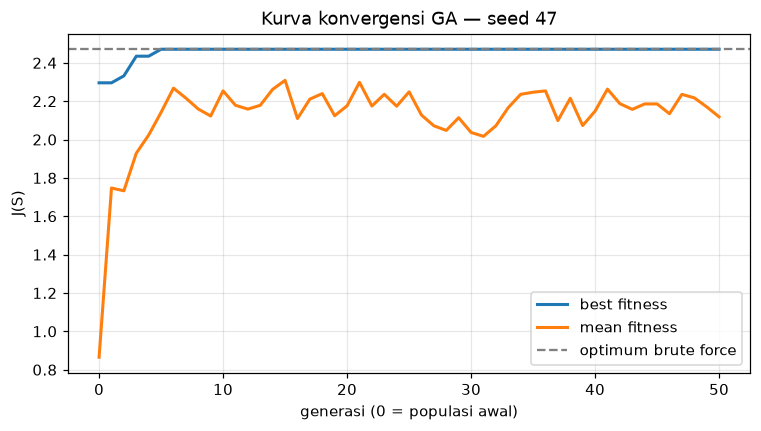
\includegraphics[width=0.49\textwidth]{figures/soal_03_3.png}\hfill
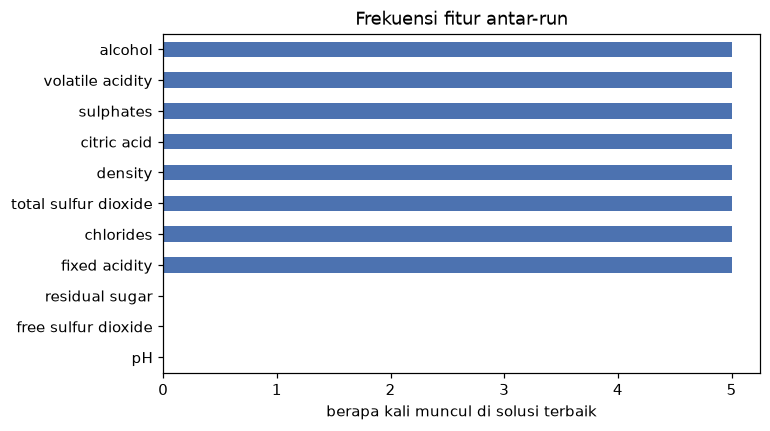
\includegraphics[width=0.46\textwidth]{figures/soal_03_4.png}
\caption{Kiri: kurva konvergensi GA seed 47; \emph{best fitness} mencapai optimum di generasi ke-5. Kanan: frekuensi fitur pada solusi terbaik dari 5 run.}
\end{figure}

\begin{adjustbox}{max width=\textwidth}\begin{tabular}{@{}lcc|lcc@{}}
\toprule
\textbf{Fitur} & \textbf{Frek.} & \textbf{Skor} & \textbf{Fitur} & \textbf{Frek.} & \textbf{Skor} \\
\midrule
alcohol & 5 & 0.964 & total sulfur dioxide & 5 & 0.239 \\
volatile acidity & 5 & 0.575 & chlorides & 5 & 0.220 \\
sulphates & 5 & 0.405 & fixed acidity & 5 & 0.185 \\
citric acid & 5 & 0.376 & residual sugar & 0 & 0.081 \\
density & 5 & 0.307 & free sulfur dioxide & 0 & 0.080 \\
 & & & pH & 0 & 0.064 \\
\bottomrule
\end{tabular}\end{adjustbox}

Tiga fitur tidak pernah terpilih karena skornya 0.06-0.08, di bawah penalti 0.10. GA sangat stabil karena $J(S)$ bisa dipecah per fitur dan ruang solusinya kecil, jadi tidak ada optimum lokal yang menjebak. Fitur yang paling tipis lolosnya adalah \emph{fixed acidity}, hanya 0.085 di atas penalti.

Stabil terhadap seed belum tentu stabil terhadap data. Kalau $J$ dihitung dari seluruh data tanpa split, \emph{free sulfur dioxide} ikut lolos dengan skor 0.127 dan hasilnya menjadi 9 fitur, padahal di data latih skornya hanya 0.080. Fitur ini berada tepat di sekitar ambang. Split tetap saya pakai supaya pemilihan fitur tidak melihat data \emph{hold-out}, sesuai petunjuk UTS no.~4.

\jawab{Jawaban 3d: Apakah fitur terpilih benar-benar terpisah?}
Skor $J$ hanya memakai mean dan std, dan mean mudah terseret outlier. Karena itu pemisahannya saya uji lagi dengan uji peringkat Mann-Whitney (tahan outlier), Kolmogorov-Smirnov (KS), dan AUC satu fitur.

\begin{adjustbox}{max width=\textwidth}\begin{tabular}{@{}lcccccc@{}}
\toprule
\textbf{Fitur} & \textbf{Terpilih} & \textbf{Median H} & \textbf{Median L} & \textbf{AUC} & \textbf{KS} & \textbf{$p$ Mann-Whitney} \\
\midrule
alcohol & ya & 11.70 & 9.70 & 0.912 & 0.691 & $1.4\times10^{-52}$ \\
volatile acidity & ya & 0.38 & 0.59 & 0.803 & 0.492 & $3.6\times10^{-29}$ \\
sulphates & ya & 0.74 & 0.58 & 0.795 & 0.521 & $8.0\times10^{-28}$ \\
fixed acidity & ya & 8.70 & 7.80 & 0.619 & 0.224 & $1.1\times10^{-5}$ \\
free sulfur dioxide & tidak & 12.0 & 15.0 & 0.560 & 0.124 & 0.027 \\
pH & tidak & 3.27 & 3.31 & 0.550 & 0.119 & 0.065 \\
\bottomrule
\end{tabular}\end{adjustbox}

\fig{soal_03_5.png}{1.0}{Distribusi H vs L: dua fitur terkuat, fitur terpilih terlemah (\emph{fixed acidity}), dan fitur tidak terpilih (pH).}

Fitur terkuat memang terpisah dengan jelas. AUC 0.91 pada \emph{alcohol} berarti 91\% kemungkinan wine bagus punya alkohol lebih tinggi dari wine jelek, dan histogram kedua kelompok hampir tidak bertumpuk. Kedelapan fitur terpilih signifikan ($p \leq 1.1\times10^{-5}$), tetapi kekuatannya berbeda: distribusi \emph{fixed acidity} (KS 0.22) masih banyak bertumpuk. Dengan ratusan sampel, perbedaan kecil pun bisa signifikan, jadi signifikan belum tentu kuat secara praktis. Fitur yang tidak dipilih memang lemah; pH bahkan tidak signifikan dan histogram H dan L-nya hampir identik.

Kelemahan $J(S)$ ada pada redundansi. \emph{Fixed acidity} berkorelasi 0.67 dengan \emph{citric acid} dan 0.63 dengan \emph{density}, sedangkan \emph{density} berkorelasi $-0.48$ dengan \emph{alcohol}. Di data \emph{hold-out}, logistic regression dengan 8 fitur GA mendapat balanced accuracy 0.826, dengan semua 11 fitur 0.822, dan dengan 3 fitur teratas saja 0.802. Sebagian fitur ternyata membawa informasi yang sama.

Jadi fitur yang sering dipilih memang memisahkan distribusi secara nyata, terutama \emph{alcohol}, \emph{volatile acidity}, dan \emph{sulphates}. Untuk perbaikan, fitness bisa diberi penalti korelasi antar-fitur terpilih seperti pada mRMR.

\subsection{Interpretasi Hasil}
Logistic regression dengan 8 fitur hasil GA, diuji pada data \emph{hold-out}, mencapai accuracy 0.848 dan balanced accuracy 0.826. Dari 37 wine berkualitas tinggi, 29 terdeteksi (recall 0.784). Kesalahan terbanyak berasal dari 17 wine biasa yang terlihat bagus, misalnya beralkohol tinggi tetapi berkualitas rendah.

\begin{adjustbox}{max width=\textwidth}\begin{tabular}{@{}llll@{}}
\toprule
\textbf{Kriteria} & \textbf{Target} & \textbf{Hasil} & \textbf{Status} \\
\midrule
GA = optimum \emph{brute force} & selisih 0 & $J = 2.4708$ (5 run) & \ok{tercapai} \\
Konsistensi antar-run & $\geq 4/5$ & 5/5 & \ok{tercapai} \\
Fitur terpilih signifikan & $p < 0.05$ & 8/8 & \ok{tercapai} \\
Separasi \emph{hold-out} & $\geq 0.75$ & 0.826 & \ok{tercapai} \\
\bottomrule
\end{tabular}\end{adjustbox}

GA biner menemukan subset optimal 8 dari 11 fitur dan memberi jawaban yang sama di semua seed, terutama karena $J(S)$ bisa dipecah per fitur dan ruang solusinya kecil. \emph{Mutation rate} 0.05 sampai 0.10 paling efisien. Kalau anggaran uji lab terbatas, \emph{alcohol}, \emph{volatile acidity}, dan \emph{sulphates} saja sudah memberi balanced accuracy 0.80.

\newpage
\section{Soal 7: Optimasi Multi-output Energy Efficiency dengan PSO}

Dataset D3 Energy Efficiency berisi 768 bangunan hasil simulasi dengan 8 fitur dan dua target, Heating Load ($Y_1$) dan Cooling Load ($Y_2$). PSO dijalankan dengan \texttt{pyswarms}.

\subsection{Business Understanding}
Sebelum gedung dibangun, arsitek perlu perkiraan beban pemanas dan pendingin untuk menentukan ukuran AC atau heater dan biaya operasionalnya. Simulasi detail itu lambat, jadi yang dicari di sini adalah semacam kalkulator kasar: dua model linear yang koefisiennya dicari PSO sekaligus dalam satu partikel.

\begin{tabularx}{\textwidth}{@{}LL@{}}
\toprule
\textbf{Kriteria kesuksesan} & \textbf{Ambang} \\
\midrule
PSO mendekati solusi analitik OLS di data latih & $J_{PSO} \leq 1.01 \times J_{OLS}$ \\
$R^2$ test masing-masing target & $\geq 0.85$ \\
Error relatif & RMSE $\leq 0.4\,\sigma$ target \\
\bottomrule
\end{tabularx}

\subsection{Data Understanding dan Data Preparation}
Data simulasi ini rapi: tidak ada missing value, duplikat, ataupun outlier menurut aturan IQR. Heating dan Cooling berkorelasi sangat kuat (0.976), dan distribusi keduanya punya dua puncak karena \emph{Overall\_Height} hanya bernilai 3.5 m atau 7 m.

Masalah terbesarnya multikolinearitas. Relative\_Compactness dan Surface\_Area berkorelasi $-0.99$, sedangkan Roof\_Area dan Overall\_Height $-0.97$. Lebih dari itu, Surface\_Area persis sama dengan Wall\_Area + 2 $\times$ Roof\_Area, sehingga rank matriks fitur hanya 7, padahal fiturnya 8.

Data dibagi 60/20/20. Train dipakai PSO, validation untuk memilih strategi batas, dan test hanya sekali di akhir. Fitur dan target distandardisasi dengan mean dan std data latih. Orientation dan Glazing\_Area\_Distribution tetap diperlakukan sebagai angka karena soal meminta model linear 8 fitur.

\fig{soal_07_1.png}{1.0}{Distribusi target, hubungan $Y_1$ dengan $Y_2$, dan Heating Load per tinggi gedung.}

\jawab{Jawaban 7a: Normalisasi RMSE dengan $\sigma$ dan dimensi partikel}
\[ J = \frac{\mathrm{RMSE}_{Y_1}}{\sigma_{Y_1}} + \frac{\mathrm{RMSE}_{Y_2}}{\sigma_{Y_2}} \]
Sebaran kedua target berbeda ($\sigma_{Y_1} = 10.07$ dan $\sigma_{Y_2} = 9.44$ di data latih). Kalau RMSE langsung dijumlahkan, target dengan angka lebih besar akan menguasai objective dan PSO hanya sibuk memperbaiki target itu. Setelah dibagi $\sigma$, RMSE menjadi ukuran ``berapa kali simpangan baku'' tanpa satuan. Nilai 1.0 berarti sama buruknya dengan selalu menebak rata-rata. Mirip nilai ujian dari dua dosen dengan skala berbeda yang harus dikonversi ke skala yang sama dulu sebelum dijumlah. Ukuran ini juga terhubung langsung dengan $R^2$ lewat $\mathrm{RMSE}/\sigma = \sqrt{1 - R^2}$.

Setiap model linear punya 8 bobot dan 1 bias, jadi satu partikel berdimensi $2 \times (8 + 1) = 18$ dengan susunan $[w^{(1)}_{1..8}, b_1, w^{(2)}_{1..8}, b_2]$.

\jawab{Jawaban 7b: Desain PSO dan \emph{boundary handling}}
Di setiap iterasi, kecepatan partikel diperbarui dari inersia, ingatan pribadi, dan tarikan kawanan:
\[ v \leftarrow w\,v + c_1 r_1 (p_{best} - x) + c_2 r_2 (g_{best} - x), \qquad x \leftarrow x + v \]

\begin{tabularx}{\textwidth}{@{}llL@{}}
\toprule
\textbf{Parameter} & \textbf{Nilai} & \textbf{Alasan} \\
\midrule
Partikel / iterasi & 40 / 300 & sekitar 2$\times$ dimensi; kurva sudah datar jauh sebelum iterasi 300 \\
$w$ & 0.7 & nilai konstan yang umum, mendekati 0.729 dari analisis Clerc \& Kennedy \\
$c_1 = c_2$ & 1.5 & ingatan pribadi dan pengaruh kawanan seimbang \\
Batas posisi & $[-3, 3]$ & data terstandardisasi, koefisien wajar sekitar $\pm$1; mencegah koefisien liar \\
Velocity clamp & $[-1, 1]$ & maksimal 1/6 lebar ruang per langkah \\
\bottomrule
\end{tabularx}

Clipping (\texttt{nearest}) menempelkan partikel yang keluar ke dinding terdekat, misalnya 3.7 menjadi 3.0. Caranya sederhana dan cocok kalau optimum ada di dekat batas, tetapi partikel bisa menumpuk di dinding sehingga keragaman swarm berkurang. Reflection (\texttt{reflective}) memantulkan partikel sejauh kelebihannya, jadi 3.7 menjadi 2.3. Partikel tetap bergerak dan keragaman terjaga, hanya saja partikel sulit diam tepat di batas kalau optimum memang ada di sana.

Keduanya saya uji dengan 5 seed per strategi:

\begin{adjustbox}{max width=\textwidth}\begin{tabular}{@{}lcccc@{}}
\toprule
& \textbf{$J$ train akhir} & \textbf{$J$ validation} & \textbf{$J$ train iterasi 20} & \textbf{Menempel di dinding (iter.~10)} \\
\midrule
Clipping & $0.6336 \pm 0.0040$ & $0.6343 \pm 0.0030$ & 1.111 & 1.2\% (puncak 4.4\%) \\
Reflection & $0.6327 \pm 0.0036$ & $0.6348 \pm 0.0035$ & 1.203 & 0\% \\
\bottomrule
\end{tabular}\end{adjustbox}

\fig{soal_07_3.png}{1.0}{Kiri: konvergensi gbest untuk 5 seed per strategi. Kanan: porsi koordinat partikel yang menempel di batas $\pm$3.}

Clipping memang membuat sebagian partikel menempel di dinding, tetapi hanya di awal pencarian dan jumlahnya kecil. Hasil akhirnya praktis sama, dengan selisih $J$ validation 0.0005, jauh di bawah variasi antar-seed. Penyebabnya, optimum OLS (sekitar $\pm$0.8) berada jauh di dalam batas $\pm$3. Strategi dipilih dari $J$ validation terkecil, yaitu clipping.

\jawab{Jawaban 7c: RMSE, $R^2$, dan \emph{convergence curve}}
\begin{adjustbox}{max width=\textwidth}\begin{tabular}{@{}lcccc@{}}
\toprule
\textbf{Target (test)} & \textbf{RMSE} & \textbf{MAE} & \textbf{$R^2$} & \textbf{RMSE/$\sigma$} \\
\midrule
Heating Load ($Y_1$) & 2.69 kWh/m$^2$ & 1.96 & 0.934 & 0.267 \\
Cooling Load ($Y_2$) & 3.27 kWh/m$^2$ & 2.18 & 0.892 & 0.346 \\
OLS pembanding (Heating / Cooling) & 2.70 / 3.28 & 1.98 / 2.20 & 0.933 / 0.891 & - \\
\bottomrule
\end{tabular}\end{adjustbox}

\begin{figure}[H]\centering
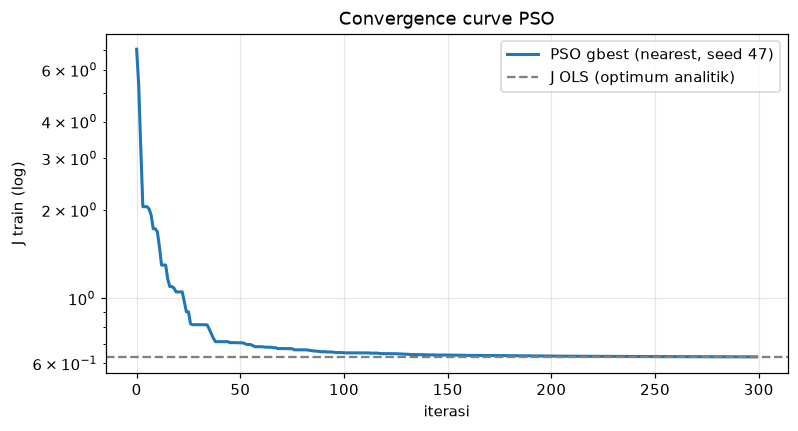
\includegraphics[width=0.42\textwidth]{figures/soal_07_4.png}\hfill
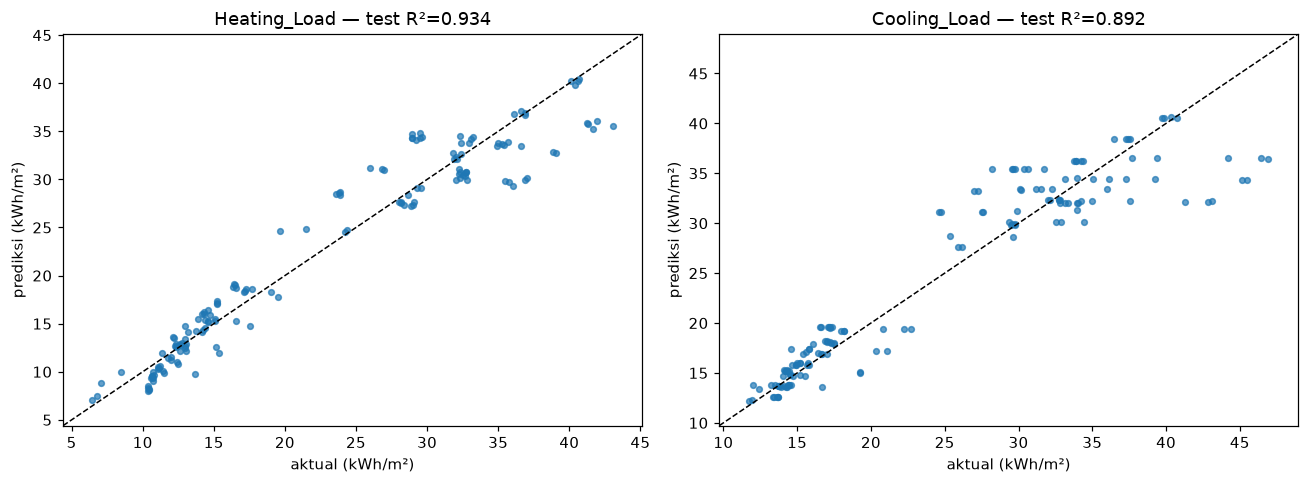
\includegraphics[width=0.56\textwidth]{figures/soal_07_5.png}
\caption{Kiri: \emph{convergence curve} PSO (seed 47) dibanding $J$ OLS. Kanan: prediksi vs aktual di test set.}
\end{figure}

$J$ test sebesar 0.613 hampir sama dengan train (0.632) dan validation (0.634), jadi model tidak overfit. PSO juga hampir mencapai optimum analitik: $J$ train 0.6321 dibanding 0.6302 milik OLS, hanya 0.3\% lebih buruk. Cooling lebih sulit diprediksi dan lebih menyebar di nilai tinggi, kemungkinan karena interaksi kaca dan tinggi gedung yang tidak bisa ditangkap model linear murni.

\jawab{Jawaban 7d: Fitur dominan dan keterbatasan interpretasi}
\begin{figure}[H]\centering
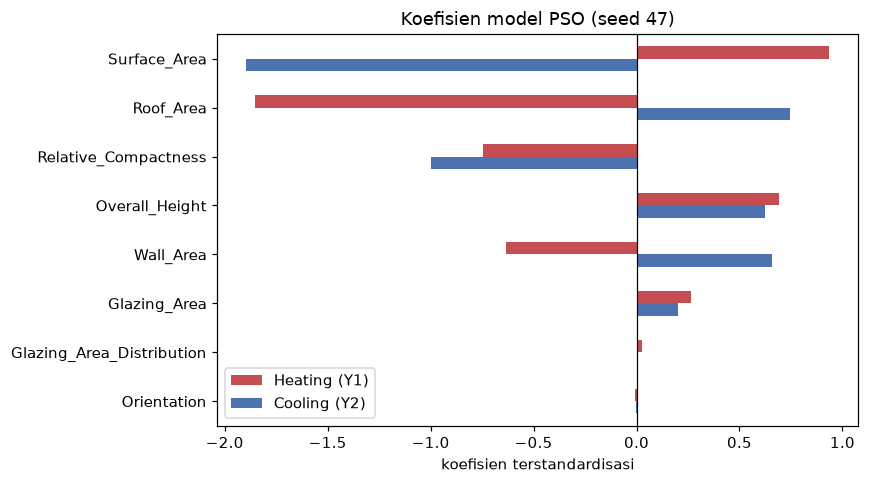
\includegraphics[width=0.55\textwidth]{figures/soal_07_6.png}
\caption{Koefisien terstandardisasi model PSO (seed 47).}
\end{figure}

\begin{adjustbox}{max width=\textwidth}\begin{tabular}{@{}lcccccc@{}}
\toprule
\textbf{Koef.\ Heating per seed} & \textbf{47} & \textbf{48} & \textbf{49} & \textbf{50} & \textbf{51} & \textbf{std} \\
\midrule
Relative\_Compactness & $-0.746$ & $-0.421$ & $-0.590$ & $0.096$ & $-0.462$ & 0.318 \\
Surface\_Area & 0.934 & $-0.445$ & 0.097 & 0.221 & $-0.933$ & 0.707 \\
Wall\_Area & $-0.632$ & 0.258 & $-0.120$ & 0.181 & 0.475 & 0.428 \\
Roof\_Area & $-1.853$ & 0.070 & $-0.733$ & 0.116 & 0.524 & 0.943 \\
Overall\_Height & 0.692 & 0.847 & 0.784 & 1.059 & 0.836 & 0.135 \\
Glazing\_Area & 0.264 & 0.265 & 0.269 & 0.275 & 0.268 & 0.004 \\
Orientation & $-0.009$ & $-0.008$ & $-0.007$ & $-0.006$ & $-0.006$ & 0.001 \\
\bottomrule
\end{tabular}\end{adjustbox}

Dua fitur bisa dipercaya sebagai fitur dominan. Overall\_Height selalu positif (0.69 sampai 1.06 di kelima seed), dan solusi OLS juga menempatkannya sebagai koefisien terbesar (+0.76 untuk Heating dan +0.80 untuk Cooling). Glazing\_Area sangat stabil dengan std antar-seed 0.004. Orientation tidak berpengaruh karena koefisiennya selalu mendekati nol.

Kalau koefisien seed 47 dibaca mentah, fitur paling dominan justru Surface\_Area dan Roof\_Area. Masalahnya, koefisien Roof\_Area bisa $-1.85$ di satu seed dan $+0.52$ di seed lain, padahal $J$ kelima seed hampir sama (0.630 sampai 0.640). Penyebabnya terlihat jelas saat koefisien (Surface, Wall, Roof) saya geser dari $(0.93, -0.63, -1.85)$ ke $(1.89, -1.12, -2.85)$: $J$ train tetap 0.632094 sampai 6 desimal. Karena Surface = Wall + 2 $\times$ Roof, ada tak terhingga kombinasi koefisien dengan prediksi yang identik. Seperti tiga orang yang mengangkat satu meja: berat totalnya selalu sama, tetapi pembagian beban per orang bisa berapa saja.

Magnitudo koefisien hanya sah dibandingkan kalau fitur-fiturnya tidak saling berkorelasi. Untuk dataset ini ada tiga jalan keluar: membuang fitur yang kolinear sempurna, menambah regularisasi L2 di objective agar solusinya unik, atau memakai \emph{permutation importance} per kelompok fitur.

\subsection{Interpretasi Hasil}
Pada 20 bangunan test, sebagian besar prediksi meleset 0 sampai 3 kWh/m$^2$. Kesalahan terbesar ada pada gedung tinggi dengan kaca 40\%, dengan Cooling aktual 46.4 dan prediksi 36.5. Ini kasus interaksi tinggi dan kaca yang tidak tertangkap model linear.

\begin{adjustbox}{max width=\textwidth}\begin{tabular}{@{}llll@{}}
\toprule
\textbf{Kriteria} & \textbf{Target} & \textbf{Hasil} & \textbf{Status} \\
\midrule
$J_{PSO} \leq 1.01\,J_{OLS}$ & $\leq 1.01$ & 1.0031 (4/5 seed; seed 50 = 1.016) & \ok{tercapai} \\
$R^2$ test Heating / Cooling & $\geq 0.85$ & 0.934 / 0.892 & \ok{tercapai} \\
RMSE $\leq 0.4\sigma$ & $\leq 0.4$ & 0.267 / 0.346 & \ok{tercapai} \\
\bottomrule
\end{tabular}\end{adjustbox}

Satu partikel 18 dimensi berhasil mengoptimasi dua model sekaligus dengan hasil yang praktis sama dengan OLS. Clipping dan reflection berakhir di model yang sama karena optimum jauh dari batas. Tinggi gedung dan luas kaca adalah fitur dominan yang bisa dipercaya, sedangkan koefisien fitur geometri lain tidak bisa ditafsirkan per fitur karena kolinear sempurna.

\newpage
\section{Soal 12: FIS Mamdani untuk Risiko Ketidakstabilan Grid}

Dataset D6 Electrical Grid Stability berisi 10.000 simulasi grid 4 node. FIS dibangun dengan \texttt{scikit-fuzzy}.

\subsection{Business Understanding}
Grid listrik terdesentralisasi bisa menjadi tidak stabil kalau pesertanya (satu pembangkit dan tiga konsumen) bereaksi terlalu lambat atau terlalu agresif terhadap perubahan harga. Operator butuh indikator risiko yang alasannya bisa dijelaskan. Fuzzy logic cocok karena aturannya ditulis dalam bahasa manusia, seperti lampu indikator di dasbor mobil yang disertai buku manual.

\begin{tabularx}{\textwidth}{@{}LL@{}}
\toprule
\textbf{Kriteria kesuksesan} & \textbf{Ambang} \\
\midrule
Rule base lengkap & 0 kombinasi tanpa rule dan 0 sampel dengan aktivasi maksimum $< 0.2$ \\
FIS lebih baik dari baseline threshold satu fitur & macro-F1 test lebih tinggi \\
Kemampuan ranking skor risiko & ROC-AUC test $\geq 0.70$ \\
\bottomrule
\end{tabularx}

\subsection{Data Understanding dan Data Preparation}
Datanya bersih dari missing value, duplikat, dan outlier, dan semua fitur menyebar seragam karena dibangkitkan simulator. Target tidak seimbang: 63.8\% sampel unstable. Daya $p_1$ selalu sama dengan $-(p_2 + p_3 + p_4)$, jadi tidak membawa informasi baru. Kolom \texttt{stab} saya buang karena \texttt{stabf} hanyalah tanda positif atau negatif dari \texttt{stab}; memakainya sebagai input sama dengan membocorkan label.

Data dibagi 60/20/20 secara berstrata. Data latih dipakai untuk memilih fitur, membangun membership, dan mengecek rule. Validation hanya dipakai untuk memilih threshold dan versi rule, dan test untuk evaluasi akhir. FIS membaca nilai asli lewat membership, jadi tidak perlu scaling.

\jawab{Jawaban 12a: Pemilihan tiga fitur, universe, dan membership}
Setiap fitur saya nilai dari data latih dengan tiga ukuran, yaitu korelasi point-biserial $|r|$, \emph{mutual information}, dan AUC satu fitur, lalu peringkat ketiganya dirata-rata.

\begin{adjustbox}{max width=\textwidth}\begin{tabular}{@{}lccccc@{}}
\toprule
\textbf{Fitur} & \textbf{$|r|$} & \textbf{MI} & \textbf{AUC} & \textbf{$p$ Mann-Whitney} & \textbf{Rata-rata peringkat} \\
\midrule
$\tau_1$ & 0.244 & 0.041 & 0.647 & $4.1\times10^{-80}$ & 1.0 \\
$\tau_4$ & 0.243 & 0.040 & 0.647 & $8.8\times10^{-80}$ & 2.0 \\
$\tau_2$ & 0.240 & 0.035 & 0.644 & $4.4\times10^{-77}$ & 3.3 \\
$g_2$ & 0.236 & 0.030 & 0.642 & $1.2\times10^{-74}$ & 4.3 \\
$p_1$-$p_4$ & $\leq 0.03$ & $\approx 0$ & $\approx 0.50$ & - & $\geq 9$ \\
\bottomrule
\end{tabular}\end{adjustbox}

Yang terpilih adalah $\tau_1$, $\tau_4$, dan $\tau_2$, yaitu waktu reaksi peserta. Kemenangannya tipis karena $g_2$ hampir setara. Universe setiap fitur adalah rentang [min, max] data latih. Low berbentuk trapesium $[\min, \min, Q_1, Q_2]$, Medium segitiga $[Q_1, Q_2, Q_3]$, dan High trapesium $[Q_2, Q_3, \max, \max]$. Dengan kuartil, batas mengikuti sebaran data asli, dan di setiap titik derajat Low, Medium, dan High berjumlah 1 (\emph{fuzzy partition}).

Output \emph{Instability Risk} memakai skala 0 sampai 100 dengan Low $[0,0,20,45]$, Medium $[25,50,75]$, dan High $[55,80,100,100]$. Ketiganya dibagi rata dan saling tumpang tindih sekitar 20 poin supaya risiko berpindah dengan halus. Bentuk output tidak saya atur dari data karena skala risiko ini buatan kita sendiri.

\fig{soal_12_2.png}{1.0}{Membership function tiga input (dari kuartil data latih) dan output.}

\jawab{Jawaban 12b: Rule base, coverage, dan deteksi \emph{rule gaps}}
Agar semua kombinasi tercakup, saya membuat rule untuk ke-27 kombinasi ($3^3$). Konsekuen versi pertama memakai poin bahaya: Low = 0, Medium = 1, High = 2, lalu dijumlahkan. Total 0 sampai 2 menjadi risiko Low, 3 menjadi Medium, dan 4 sampai 6 menjadi High.

Saat dicek dengan data latih, rentang porsi unstable antar-konsekuen ternyata tumpang tindih. Rule Medium-Medium-Medium diberi konsekuen Medium, padahal porsi unstable-nya 0.934 dan termasuk yang tertinggi. Plot per desil menunjukkan alasannya: pengaruh $\tau$ jenuh. Porsi unstable naik tajam dari sekitar 0.33 sampai sekitar 0.70 di dekat median, lalu mendatar. Bagi stabilitas, $\tau$ Medium sudah sama berbahayanya dengan High.

Rule versi kedua saya susun ulang dari data latih berdasarkan jumlah input yang Low. Tidak ada input Low berarti risiko High, satu input Low berarti Medium, dan dua atau lebih berarti Low. Analoginya rem mobil: telat setengah detik atau dua detik sama-sama sudah terlambat, dan yang menolong hanya rem yang responsnya cepat.

\fig{soal_12_3.png}{1.0}{Porsi unstable per desil fitur (data latih). Efeknya jenuh setelah sekitar median.}

\begin{adjustbox}{max width=\textwidth}\begin{tabular}{@{}lccc@{}}
\toprule
\textbf{Konsekuen v2} & \textbf{Jumlah rule} & \textbf{Porsi unstable (min-maks)} & \textbf{Rata-rata} \\
\midrule
Low ($\geq$2 input Low) & 7 & 0.217 - 0.473 & 0.390 \\
Medium (1 input Low) & 12 & 0.602 - 0.757 & 0.668 \\
High (0 input Low) & 8 & 0.833 - 0.935 & 0.899 \\
\bottomrule
\end{tabular}\end{adjustbox}

Rule gaps saya deteksi dengan dua cara. Pertama secara struktural, dengan memastikan setiap kombinasi punya rule. Kedua secara empiris, dengan menghitung aktivasi rule terkuat (min derajat antecedent) untuk setiap sampel latih; sampel dengan aktivasi di bawah 0.2 berarti tidak dikenali rule mana pun. Rule base 27 rule tidak menyisakan kombinasi kosong, dan aktivasi terendahnya 0.50 di keenam ribu sampel. Untuk membuktikan detektornya bekerja, sembilan rule dengan $\tau_1$ = Medium sengaja saya hapus. Detektor langsung menemukan 9 kombinasi kosong dan 608 sampel dengan aktivasi di bawah 0.2.

\jawab{Jawaban 12c: Implementasi Mamdani dan threshold dari validation}
Nilai $\tau$ mula-mula diubah menjadi derajat Low, Medium, dan High (fuzzification). Setiap rule lalu menghitung firing strength sebagai nilai min dari antecedent-nya, dan himpunan output rule itu dipotong setinggi firing strength tersebut. Potongan dari 27 rule digabung dengan operator max, lalu titik berat gabungannya (centroid) menjadi risk 0 sampai 100. Sampel dinyatakan unstable kalau risk $\geq \theta$, dan $\theta$ dicari dari 0 sampai 100 untuk memaksimalkan macro-F1 di validation.

\begin{adjustbox}{max width=\textwidth}\begin{tabular}{@{}lccc@{}}
\toprule
\textbf{Versi} & \textbf{$\theta$ terbaik} & \textbf{macro-F1 val} & \textbf{ROC-AUC val} \\
\midrule
Rule v1 & 37.5 & 0.675 & 0.726 \\
Rule v2 (dipilih) & 39.0 & 0.690 & 0.765 \\
\bottomrule
\end{tabular}\end{adjustbox}

\begin{figure}[H]\centering
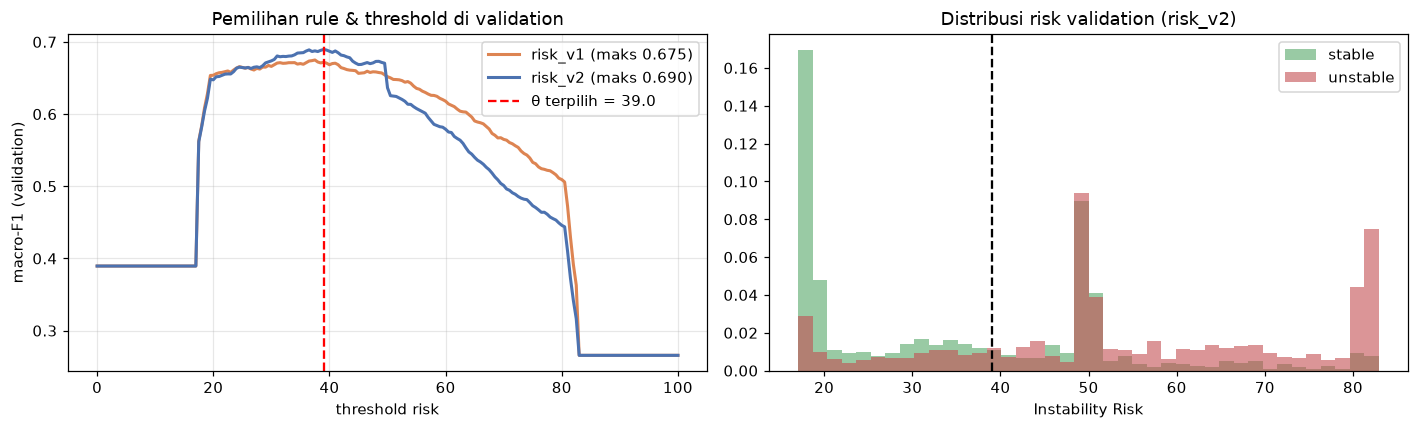
\includegraphics[width=0.62\textwidth]{figures/soal_12_5.png}\hfill
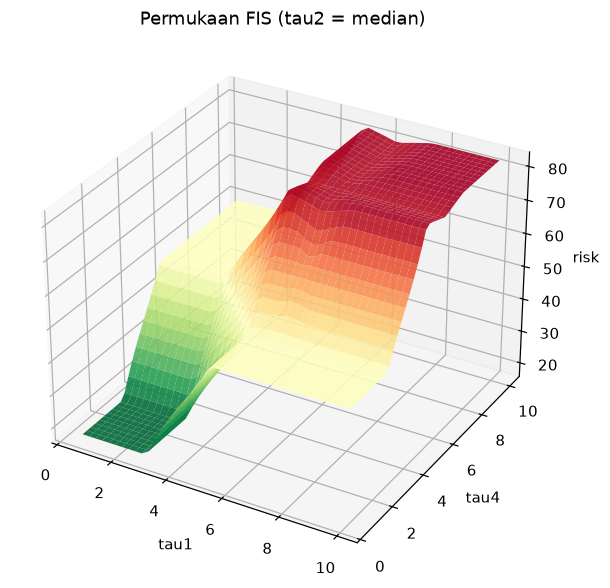
\includegraphics[width=0.36\textwidth]{figures/soal_12_6.png}
\caption{Kiri: pemilihan versi rule dan threshold di validation, serta distribusi risk. Kanan: permukaan FIS ($\tau_2$ = median).}
\end{figure}

\jawab{Jawaban 12d: Perbandingan dengan baseline threshold sederhana}
Baseline-nya satu aturan, ``unstable jika $\tau_1 \geq 3.16$'', dengan batas dipilih dari validation dengan cara yang sama. Logistic regression saya tambahkan sebagai pembanding model statistik.

\begin{adjustbox}{max width=\textwidth}\begin{tabular}{@{}lcccccc@{}}
\toprule
\textbf{Model (test)} & \textbf{Acc} & \textbf{Bal.\ acc} & \textbf{Macro-F1} & \textbf{Recall unst.} & \textbf{Spec.} & \textbf{AUC} \\
\midrule
Baseline $\tau_1 \geq 3.16$ & 0.676 & 0.623 & 0.626 & 0.816 & 0.430 & 0.626 \\
FIS Mamdani v2 & 0.720 & 0.690 & 0.692 & 0.798 & 0.582 & 0.778 \\
Logistic regression & 0.693 & 0.681 & 0.676 & 0.724 & 0.638 & 0.754 \\
\bottomrule
\end{tabular}\end{adjustbox}

Baseline hanya punya satu saklar, sehingga untuk mengejar recall tinggi ia terpaksa menuduh banyak grid stabil sebagai unstable (specificity 0.43). FIS unggul di semua metrik gabungan, dengan macro-F1 lebih tinggi 0.066 dan AUC lebih tinggi 0.15. FIS bahkan sedikit di atas logistic regression, karena rule v2 menangkap efek jenuh yang oleh logistic regression dianggap lurus.

Dari sisi interpretabilitas, setiap keputusan FIS bisa ditelusuri ke rule yang aktif. Sampel dengan $\tau = (9.75, 9.71, 7.65)$, misalnya, mendapat risk 82.9 karena rule ``IF semua High THEN risk High'' aktif 100\%. Rule juga bisa diubah pakar tanpa melatih ulang model. Kekurangannya, skor risk berundak dan sering tepat 17.1, 50, atau 82.9, dan FIS hanya melihat 3 dari 12 fitur sehingga elastisitas $g$ tidak ikut diperhitungkan.

FIS tetap lebih layak walau akurasinya sedikit lebih rendah ketika keputusan harus bisa diaudit, misalnya saat operator harus menjelaskan alasan pelepasan beban. FIS juga cocok ketika data sedikit tetapi ada pengetahuan pakar, ketika yang dibutuhkan peringatan bertingkat (hijau, kuning, merah) dan bukan sekadar ya atau tidak, dan ketika perilaku model harus bisa diperiksa di seluruh ruang input lewat permukaan FIS dan cek celah rule.

\subsection{Interpretasi Hasil}
Dari 20 sampel test, 14 ditebak benar, dengan 4 false alarm dan 2 grid unstable yang terlewat. Tiga dari empat false alarm punya risk sekitar 50, yaitu zona abu-abu yang porsi unstable-nya sekitar 0.67.

\begin{adjustbox}{max width=\textwidth}\begin{tabular}{@{}llll@{}}
\toprule
\textbf{Kriteria} & \textbf{Target} & \textbf{Hasil} & \textbf{Status} \\
\midrule
Rule base lengkap & 0 kosong, 0 aktivasi $< 0.2$ & 0 dan 0 (min 0.50) & \ok{tercapai} \\
FIS $>$ baseline & macro-F1 test & 0.692 vs 0.626 & \ok{tercapai} \\
Ranking skor risk & AUC $\geq 0.70$ & 0.778 & \ok{tercapai} \\
\bottomrule
\end{tabular}\end{adjustbox}

Validasi rule dengan data latih membuktikan bahwa asumsi awal saya keliru: waktu reaksi yang makin lama tidak membuat grid makin berbahaya secara lurus. Rule yang disusun ulang berdasarkan jumlah peserta yang bereaksi cepat lebih akurat dan tetap mudah dibaca. Langkah berikutnya bisa menambah input $g$ lewat hierarchical FIS atau menyetel membership dengan ANFIS.

\newpage
\section{Soal 16: MLP untuk Prediksi Horsepower (Auto MPG)}

Dataset D8 Auto MPG berisi 398 mobil keluaran 1970 sampai 1982. Model dibangun dengan \texttt{PyTorch}.

\subsection{Business Understanding}
Data spesifikasi kendaraan sering bolong, termasuk horsepower yang dipakai untuk pajak, asuransi, dan perbandingan performa. Kalau horsepower bisa ditebak akurat dari spesifikasi lain, data yang bolong bisa dilengkapi. Seperti montir berpengalaman yang bisa menebak tenaga mesin dari ukuran mesin dan bobot mobil.

\begin{tabularx}{\textwidth}{@{}LL@{}}
\toprule
\textbf{Kriteria kesuksesan} & \textbf{Ambang} \\
\midrule
$R^2$ test & $\geq 0.85$ \\
MAE test & $\leq 10$ hp \\
Tidak overfit berat & RMSE test $\leq 1.3 \times$ RMSE train \\
Lebih baik dari atau setara regresi linear & RMSE test MLP $\leq$ linear \\
\bottomrule
\end{tabularx}

\subsection{Data Understanding}
Dari 398 mobil tidak ada duplikat. Missing value hanya ada di horsepower, sebanyak 6 baris: Ford Pinto, Ford Maverick, Renault LeCar, Ford Mustang Cobra, Renault 18i, dan AMC Concord. Horsepower berkisar 46 sampai 230 hp (rata-rata 104, std 38.5) dan miring ke kanan. Ke-10 outlier IQR semuanya mobil V8 bertenaga besar, bukan salah input.

Horsepower berhubungan kuat dengan fitur lain: korelasinya 0.90 dengan displacement, 0.87 dengan weight, 0.84 dengan cylinders, $-0.78$ dengan mpg, dan $-0.69$ dengan acceleration. Scatter horsepower terhadap mpg melengkung, jadi MLP yang bisa menangkap pola non-linear layak dicoba.

\fig{soal_16_1.png}{0.95}{Distribusi horsepower dan hubungannya dengan fitur lain (warna = origin).}

\jawab{Jawaban 16a: Preprocessing dan urutan agar tidak bocor}
\begin{tabularx}{\textwidth}{@{}lp{2.6cm}L@{}}
\toprule
\textbf{Langkah} & \textbf{Kapan / dari mana} & \textbf{Alasan} \\
\midrule
1. Hapus 6 baris horsepower kosong & sebelum split (sesuai soal) & horsepower adalah target, dan mengisinya dengan mean sama dengan mengarang kunci jawaban. Menghapus tidak menghitung statistik apa pun, jadi aman dilakukan sebelum split. \\
2. Buang \texttt{car\_name} & sebelum split & sesuai soal; teks unik per mobil \\
3. Split 70/15/15 (seed 47) & - & 274 train, 59 validation, 59 test \\
4. One-hot \texttt{origin} (USA/Eropa/Jepang) & kategori tetap & angka 1/2/3 hanya kode; kalau dibiarkan numerik, model mengira Jepang = 3$\times$ USA \\
5. StandardScaler 6 fitur numerik & fit di train saja & MLP sensitif skala (berat sekitar 3000, silinder sekitar 5); statistik test tidak boleh dipakai \\
6. Standardisasi target & mean/std train & gradien lebih stabil; prediksi dikembalikan ke satuan hp sebelum metrik dihitung \\
\bottomrule
\end{tabularx}

\emph{Data leakage} mirip siswa yang sudah melihat soal ujian saat belajar: nilainya bagus, tetapi tidak menggambarkan pemahaman. Outlier tidak saya buang karena mobil V8 bertenaga besar memang ada, dan model perlu belajar dari mereka.

\jawab{Jawaban 16b: Rancangan MLP}
Arsitekturnya \texttt{input(9) $\to$ Linear(64) $\to$ ReLU $\to$ Linear(32) $\to$ ReLU $\to$ Linear(1)} dengan 2.753 parameter.

\begin{tabularx}{\textwidth}{@{}llL@{}}
\toprule
\textbf{Komponen} & \textbf{Pilihan} & \textbf{Alasan} \\
\midrule
Hidden layer & 64 dan 32 neuron & memenuhi syarat minimal 2 hidden layer; bentuk corong dengan ukuran wajar untuk 274 data \\
Aktivasi & ReLU & cepat, gradien tidak menghilang, bisa menangkap pola melengkung \\
Output & 1 neuron linear & regresi, jadi output berupa angka bebas \\
Loss & MSE & standar regresi dan sejalan dengan RMSE \\
Optimizer & Adam, lr 0.001, batch 32 & menyesuaikan langkah tiap bobot, stabil untuk data kecil \\
Early stopping & patience 100, maks 3000 epoch & ambil bobot dengan RMSE validation terbaik \\
\bottomrule
\end{tabularx}

\jawab{Jawaban 16c: Hasil, \emph{learning curve}, dan prediksi vs aktual}
\begin{adjustbox}{max width=\textwidth}\begin{tabular}{@{}lccc@{}}
\toprule
\textbf{Data} & \textbf{MAE (hp)} & \textbf{RMSE (hp)} & \textbf{$R^2$} \\
\midrule
MLP train & 7.48 & 10.63 & 0.927 \\
MLP validation & 6.30 & 9.05 & 0.948 \\
MLP test & 5.40 & 7.10 & 0.951 \\
Regresi linear test & 6.51 & 7.82 & 0.941 \\
\bottomrule
\end{tabular}\end{adjustbox}

\fig{soal_16_2.png}{1.0}{Kiri: \emph{learning curve} dengan bobot terbaik di epoch 28. Kanan: prediksi vs aktual di test set.}

Di test set, MLP rata-rata meleset 5.4 hp dan menjelaskan 95.1\% variasi horsepower. MAE-nya sekitar 17\% lebih kecil dari regresi linear. Setelah kira-kira epoch 25, RMSE validation mendatar di sekitar 9 hp sementara RMSE train terus turun, tanda model mulai menghafal. Early stopping mengambil bobot epoch 28, sebelum hafalan itu terjadi. Penyebaran prediksi terbesar ada pada mobil V8 140 sampai 200 hp.

\jawab{Jawaban 16d: Overfit atau underfit, dan eksperimen satu perubahan}
Model ini tidak overfit. RMSE train (10.6) malah lebih besar dari validation (9.0) dan test (7.1). Porsi mobil di atas 202 hp hampir sama di train (2.9\%) dan validation (3.4\%), jadi penyebabnya bukan data latih yang lebih sulit. Ada tiga hal yang menjelaskannya. Saat bobot terbaik diambil di epoch 28, model belum selesai mempelajari data latih. RMSE validation sedikit optimis karena epoch terbaik justru dipilih berdasarkan validation. Test set kebetulan lebih mudah: tidak ada satu pun mobil di atas 202 hp, dan std-nya 32.5 dibanding 39.5 di train.

Untuk eksperimen, saya mengubah satu elemen saja: menambah Dropout 0.2 setelah tiap hidden layer. Dropout mematikan 20\% neuron secara acak selama latihan, mirip belajar kelompok yang anggotanya bergantian absen sehingga semua terpaksa paham materinya. Kedua varian diulang dengan 5 seed:

\begin{adjustbox}{max width=\textwidth}\begin{tabular}{@{}lcccccc@{}}
\toprule
\textbf{Varian} & \textbf{RMSE train} & \textbf{RMSE val} & \textbf{RMSE test} & \textbf{MAE test} & \textbf{$R^2$ test} & \textbf{Epoch terbaik} \\
\midrule
Awal & $9.71 \pm 0.74$ & $9.06 \pm 0.17$ & $7.35 \pm 0.37$ & $5.71 \pm 0.34$ & 0.948 & 47 \\
Dropout 0.2 & $8.99 \pm 0.79$ & $8.86 \pm 0.38$ & $6.97 \pm 0.30$ & $5.48 \pm 0.25$ & 0.953 & 128 \\
\bottomrule
\end{tabular}\end{adjustbox}

\fig{soal_16_3.png}{0.95}{Learning curve model awal vs Dropout 0.2 (seed 47).}

Dropout menurunkan RMSE validation, yang menjadi dasar pemilihan, dan RMSE test ikut turun. Latihan menjadi lebih berisik sehingga model tidak cepat menghafal, dan bobot terbaik baru tercapai di sekitar epoch 128, jauh setelah epoch 47 pada model awal. Perbaikannya kecil, 0.2 sampai 0.4 hp, kira-kira sebesar satu simpangan baku antar-seed. Karena itu eksperimen ini saya ulang 5 seed; dengan satu seed saja kesimpulannya bisa terbalik.

\subsection{Interpretasi Hasil}
Pada 20 mobil test, kebanyakan prediksi meleset kurang dari 7 hp. Ford Galaxie 500, misalnya, punya horsepower 198 dan diprediksi 197.9. Error terbesar ada pada Ford LTD (+15 hp). Test set tidak memuat mobil di atas 202 hp, jadi kemampuan model untuk mobil bertenaga sangat besar belum benar-benar teruji. Untuk enam mobil tanpa label, semua prediksi masuk rentang horsepower mobil latih dengan jumlah silinder yang sama; Renault LeCar diprediksi 57 hp dan Ford Mustang Cobra 101 hp.

\begin{adjustbox}{max width=\textwidth}\begin{tabular}{@{}llll@{}}
\toprule
\textbf{Kriteria} & \textbf{Target} & \textbf{Hasil} & \textbf{Status} \\
\midrule
$R^2$ test & $\geq 0.85$ & 0.951 & \ok{tercapai} \\
MAE test & $\leq 10$ hp & 5.40 hp & \ok{tercapai} \\
Tidak overfit berat & $\leq 1.3\times$ train & 7.10 $\leq$ 13.8 & \ok{tercapai} \\
$\leq$ regresi linear & RMSE & 7.10 $<$ 7.82 & \ok{tercapai} \\
\bottomrule
\end{tabular}\end{adjustbox}

Dengan pipeline tanpa kebocoran, MLP 9-64-32-1 mencapai MAE 5.4 hp dan $R^2$ 0.951 tanpa overfit, berkat early stopping. Dropout 0.2 memberi perbaikan kecil tetapi konsisten. Datanya kecil, jadi \emph{k-fold cross-validation} akan memberi estimasi performa yang lebih stabil.

\newpage
\section{Soal 23: PSO-CNN untuk Hyperparameter Human Activity Recognition}

Dataset D9 Human Activity Recognition Using Smartphones berasal dari 30 relawan dengan sensor 50 Hz dan window 128 sampel. Saya memakai \texttt{pyswarms} dan \texttt{PyTorch}. Task-nya sama dengan Soal 17, yaitu 1D-CNN pada sinyal inertial mentah dengan split subjek bawaan, tetapi hyperparameter-nya dicari PSO.

\subsection{Business Understanding}
Pengenalan aktivitas dari sensor HP dipakai untuk aplikasi kesehatan, pemantauan lansia, dan kebugaran. Performa 1D-CNN bergantung pada hyperparameter, dan mencoba semua kombinasi lewat \emph{grid search} sangat mahal. PSO lebih hemat, seperti mencari warung terenak bersama teman-teman yang saling berbagi info lewat grup chat, alih-alih mendatangi semua warung satu per satu.

\begin{tabularx}{\textwidth}{@{}LL@{}}
\toprule
\textbf{Kriteria kesuksesan} & \textbf{Ambang} \\
\midrule
Accuracy dan macro-F1 test CNN hasil PSO & $\geq 0.88$ \\
PSO vs baseline manual & macro-F1 test rata-rata (3 seed) $\geq$ baseline \\
Anggaran tuning & $\leq 30$ evaluasi kandidat, $\leq 25$ menit \\
\bottomrule
\end{tabularx}

\subsection{Data Understanding dan Data Preparation}
Data latih berisi 7.352 window dari 21 subjek, dan data test 2.947 window dari 9 subjek lain. Saya memakai 6 channel: \emph{body\_acc} dan \emph{body\_gyro}, masing-masing sumbu x, y, dan z. Tidak ada NaN maupun window duplikat. Lonjakan dengan $|z| > 5$ hanya 0.21\% titik dan berasal dari hentakan kaki asli, jadi tetap dipakai. Jumlah window per kelas cukup seimbang, 986 sampai 1.407.

Sinyal aktivitas statis (duduk, berdiri, berbaring) hampir datar dan mirip satu sama lain, karena gravitasi sudah dibuang dari \emph{body\_acc}.

\fig{soal_23_2.png}{1.0}{Contoh satu window sinyal mentah untuk setiap aktivitas.}

\jawab{Jawaban 23a: Tensor, split subjek, vektor posisi, mapping, batas, dan velocity clamp}
Input \texttt{Conv1d} berformat \emph{channel-first}, yaitu (B, 6, 128). Enam sumbu sensor diperlakukan seperti enam warna pada gambar, dan kernel bergeser di sepanjang 128 titik waktu.

Split harus per subjek karena setiap orang punya gaya bergerak sendiri dan window yang berurutan saling tumpang tindih 50\%. Kalau window diacak, test set akan berisi kembaran window latih, dan model akan mengenali orangnya, bukan aktivitasnya. Karena itu test memakai 9 subjek bawaan, dan validation untuk fitness memakai 5 subjek train (7, 8, 21, 25, 26) yang dipisah dengan \texttt{GroupShuffleSplit}. Normalisasi per channel memakai mean dan std data latih saja.

Vektor posisi berdimensi 5, dan semua dimensinya dinormalisasi ke [0, 1] supaya satu velocity clamp adil untuk semua dimensi:

\begin{adjustbox}{max width=\textwidth}\begin{tabular}{@{}llll@{}}
\toprule
\textbf{Dim} & \textbf{Hyperparameter} & \textbf{Pilihan valid} & \textbf{Mapping dari $x \in [0,1]$} \\
\midrule
$x_0$ & filter F & \{16, 32, 64, 128\} & indeks = $\min(\lfloor 4x \rfloor, 3)$ \\
$x_1$ & kernel K & \{3, 5, 7, 9, 11\} & indeks = $\min(\lfloor 5x \rfloor, 4)$ \\
$x_2$ & dropout & $[0, 0.5]$ & $0.5x$ \\
$x_3$ & dense D & \{32, 64, 128, 256\} & indeks = $\min(\lfloor 4x \rfloor, 3)$ \\
$x_4$ & learning rate & $10^{u}$, $u \in [-4, -2]$ & $u = -4 + 2x$ \\
\bottomrule
\end{tabular}\end{adjustbox}

Posisi kontinu dibagi menjadi laci-laci selebar sama dan baru dibulatkan ke pilihan valid saat dievaluasi. Learning rate dicari di skala log agar ketiga orde besaran terjelajahi merata. Batas [0, 1] memakai clipping (\texttt{nearest}). Velocity clamp $[-0.25, 0.25]$ membatasi pergeseran partikel kira-kira satu laci per iterasi, supaya dengan hanya 5 iterasi partikel tidak melompat bolak-balik. Parameter PSO-nya $w = 0.7$ dan $c_1 = c_2 = 1.5$.

Kerangka CNN-nya tetap, dan ukurannya yang dicari PSO:
\begin{center}\small
\texttt{Conv1d(6$\to$F, K) $\to$ ReLU $\to$ MaxPool(2)} \quad (B, F, 64)\\
\texttt{Conv1d(F$\to$F, K) $\to$ ReLU $\to$ MaxPool(2)} \quad (B, F, 32)\\
\texttt{Flatten(F$\times$32) $\to$ Dense(D) $\to$ ReLU $\to$ Dropout $\to$ Dense(6)}
\end{center}
Panjang sequence berkurang dari 128 ke 64, lalu ke 32.

\jawab{Jawaban 23b: Fitness dan alasan macro-F1}
\[ \text{fitness} = \big(1 - \text{macro-F1}_{val}\big) + 0.02 \cdot \frac{\#\text{parameter}}{10^6} \]
Macro-F1 menghitung F1 per kelas lalu merata-ratakannya dengan bobot sama, jadi setiap aktivitas sama penting. Accuracy bisa tetap tinggi walau duduk dan berdiri selalu tertukar, sedangkan macro-F1 akan turun jelas. Penalti parameter menghargai 1 juta parameter setara 0.02 macro-F1, sehingga model besar hanya dipilih kalau macro-F1-nya setidaknya 2 poin lebih tinggi. Untuk aplikasi di HP, \emph{trade-off} ini masuk akal. Setiap kandidat dilatih dengan Adam, batch 64, maksimal 8 epoch, early stopping patience 2, dan seed yang sama.

\jawab{Jawaban 23c: PSO dengan anggaran terbatas}
Anggarannya 6 partikel $\times$ 5 iterasi = 30 evaluasi. Sebagai perbandingan, grid search kasar dengan 3 nilai dropout dan 3 nilai learning rate saja sudah butuh 720 pelatihan.

\fig{soal_23_3.png}{1.0}{Kiri: trajectory gbest dan fitness tiap partikel. Tengah: akurasi vs ukuran model. Kanan: pengaruh learning rate.}

Konfigurasi terbaik yang ditemukan adalah F = 128, K = 11, dropout 0.017, dense 32, dan lr sekitar $1.6\times10^{-3}$, dengan 320.230 parameter, macro-F1 val 0.9475, dan fitness 0.0589. Kernel 11 sampel setara sekitar 0.22 detik, cukup panjang untuk menangkap satu hentakan langkah.

Gbest bertahan di 0.0756 selama iterasi 0 sampai 2 dan turun ke 0.0589 di iterasi 3. Sebaran fitness partikel menyempit dari 0.08-0.22 menjadi 0.07-0.12. Sejak iterasi 1 hampir semua partikel memilih F = 128, sedangkan kernel baru mengumpul di 9 sampai 11 mulai iterasi 2 dan 3. Model terbesar (1.2 juta parameter, dense 256) hanya mencapai macro-F1 0.917, dan penalti parameter mendorong dense ke 32.

Fitness-nya berisik. Kandidat nomor 15 dan 20 praktis identik (dropout 0.014 dan 0.017, lr 0.0016, seed sama), tetapi macro-F1 val-nya 0.919 dan 0.948. Sebagian keunggulan gbest kemungkinan faktor beruntung (\emph{winner's curse}); saat dilatih ulang, macro-F1 val rata-ratanya 0.943. Ke-30 kandidat unik ini menghabiskan 43.2 menit, dengan kandidat F = 128, K = 11 memakan 80 sampai 180 detik masing-masing di CPU.

\jawab{Jawaban 23d: CNN hasil PSO vs baseline manual}
Baseline manualnya F = 32, K = 5, dropout 0.3, dense 64, dan lr 0.001. Kedua model dilatih ulang dengan maksimal 30 epoch, patience 5, dan 3 seed (47, 48, 49). Test dievaluasi sekali per model per seed.

\begin{adjustbox}{max width=\textwidth}\begin{tabular}{@{}lccccc@{}}
\toprule
\textbf{Model} & \textbf{Parameter} & \textbf{Waktu latih} & \textbf{macro-F1 val} & \textbf{Acc test} & \textbf{macro-F1 test} \\
\midrule
Baseline manual & 72.134 & $49 \pm 10$ s & 0.930 & $0.908 \pm 0.014$ & $0.909 \pm 0.015$ \\
PSO terbaik & 320.230 & $181 \pm 30$ s & 0.943 & $0.926 \pm 0.005$ & $0.928 \pm 0.005$ \\
\bottomrule
\end{tabular}\end{adjustbox}

\fig{soal_23_4.png}{1.0}{Confusion matrix test (seed 47): baseline manual vs CNN hasil PSO.}

Model hasil PSO unggul 1.85 poin macro-F1 dan variasinya antar-seed tiga kali lebih kecil. Ketiga seed PSO berada di atas rata-rata baseline. Perbaikan terbesar ada pada aktivitas berjalan: baseline salah mengira 46 window naik tangga sebagai turun tangga, sedangkan model PSO hanya 2. Kernel yang lebih panjang dan filter yang lebih banyak mampu menangkap ritme langkah yang bedanya tipis.

Postur statis tidak membaik. Pasangan yang paling sering tertukar pada model PSO adalah duduk ke berdiri (31), berbaring ke berdiri (31), dan berbaring ke duduk (29). Yang membedakan ketiga postur itu adalah orientasi HP terhadap gravitasi, dan komponen gravitasi sudah tidak ada di \emph{body\_acc}. Tuning hyperparameter tidak bisa memunculkan informasi yang tidak ada di input.

\begin{adjustbox}{max width=\textwidth}\begin{tabular}{@{}lll@{}}
\toprule
\textbf{Biaya} & \textbf{Baseline} & \textbf{PSO} \\
\midrule
Tuning & 0 & 43.2 menit (30 pelatihan, sekitar 53$\times$ satu latihan baseline) \\
Ukuran model & 72 ribu & 320 ribu (4.4$\times$) \\
Waktu latih final & 49 s & 181 s (3.7$\times$) \\
Keuntungan & - & +1.85 poin macro-F1, variasi 3$\times$ lebih kecil \\
\bottomrule
\end{tabular}\end{adjustbox}

Untuk riset atau prototipe, biaya ini sepadan. Empat puluh tiga menit di laptop masih murah, dan dari log PSO terlihat bahwa kernel panjang membantu sedangkan dense besar tidak perlu. Untuk aplikasi HP perlu ditimbang lagi, karena modelnya 4.4 kali lebih besar hanya untuk tambahan kurang dari 2 poin. Peningkatan yang lebih besar kemungkinan datang dari menambah channel \emph{total\_acc} ke input, bukan dari menambah anggaran tuning.

\subsection{Interpretasi Hasil}
Pada 20 window acak dari subjek test, CNN hasil PSO menebak benar semuanya, sedangkan baseline salah satu kali (berdiri ditebak duduk). Di seluruh test set, model PSO salah pada sekitar 7\% window, dan sebagian besar kesalahannya terjadi di antara tiga postur statis.

\begin{adjustbox}{max width=\textwidth}\begin{tabular}{@{}llll@{}}
\toprule
\textbf{Kriteria} & \textbf{Target} & \textbf{Hasil} & \textbf{Status} \\
\midrule
Acc / macro-F1 test PSO & $\geq 0.88$ & 0.926 / 0.928 & \ok{tercapai} \\
PSO $\geq$ baseline & macro-F1 test & 0.928 vs 0.909 & \ok{tercapai} \\
Evaluasi kandidat & $\leq 30$ & 30 & \ok{tercapai} \\
Waktu tuning & $\leq 25$ menit & 43.2 menit & \bad{tidak tercapai} \\
\bottomrule
\end{tabular}\end{adjustbox}

Hyperparameter campuran diskret dan kontinu bisa dioptimasi PSO dengan menormalisasi posisi ke [0, 1] dan memetakannya ke laci pilihan valid. Model hasil PSO mencapai macro-F1 test 0.928, lebih tinggi dan lebih stabil dari baseline, walau waktu tuningnya melewati target. Kesalahan pada postur statis perlu diatasi dengan menambah channel \emph{total\_acc}.

\newpage
\section{Penutup}

\begin{tabularx}{\textwidth}{@{}lL@{}}
\toprule
\textbf{Soal} & \textbf{Temuan utama} \\
\midrule
3 (GA) & GA menemukan optimum global (8 fitur, $J = 2.4708$) di semua seed, dan \emph{mutation rate} 0.05 sampai 0.10 paling efisien. $J(S)$ tidak memperhitungkan redundansi antar-fitur, dan \emph{free sulfur dioxide} yang skornya di sekitar ambang bisa masuk atau keluar tergantung sampel data. \\
7 (PSO) & Satu partikel 18 dimensi menyamai OLS ($R^2$ 0.934 dan 0.892). Clipping dan reflection berakhir di model yang sama. Koefisien geometri tidak bisa ditafsirkan per fitur karena Surface = Wall + 2$\times$Roof. \\
12 (Fuzzy) & Data latih menunjukkan bahwa efek $\tau$ jenuh. Rule yang direvisi mencapai macro-F1 0.692 dan AUC 0.778, mengalahkan baseline dan sedikit di atas logistic regression, dan setiap keputusannya tetap bisa dijelaskan. \\
16 (NN) & MLP mencapai MAE 5.4 hp dan $R^2$ 0.951 tanpa overfit. Dropout 0.2 memberi perbaikan kecil yang konsisten di 5 seed. \\
23 (Gabungan) & PSO-CNN mencapai macro-F1 0.928 dibanding 0.909 dan lebih stabil, dengan model 4.4$\times$ lebih besar dan tuning 43 menit. Akurasinya dibatasi oleh input yang tidak memuat gravitasi. \\
\bottomrule
\end{tabularx}

Beberapa temuan paling berguna di UTS ini baru terlihat setelah hasilnya saya periksa ulang. Fitness Soal 3 ternyata bisa dipecah per fitur, sehingga GA pasti menemukan optimumnya. Di Soal 7 ada fitur yang kolinear sempurna, di Soal 12 efek waktu reaksi ternyata jenuh, test set Soal 16 kebetulan tidak memuat mobil bertenaga besar, dan input Soal 23 kehilangan informasi gravitasi. Tanpa pemeriksaan itu, angka-angka di atas akan terlihat lebih meyakinkan daripada yang sebenarnya.

\appendix
\newpage
\section{Lampiran: Potongan Kode Inti}
Kode lengkap ada di notebook masing-masing soal. Potongan di bawah ini memuat inti mekanisme algoritmanya.

\subsection*{A. Soal 3: Fitness $J(S)$ dan konfigurasi GA (\texttt{pygad})}
\begin{lstlisting}
mu_H, mu_L = X_tr[y_tr == 1].mean(), X_tr[y_tr == 0].mean()
sd_H, sd_L = X_tr[y_tr == 1].std(), X_tr[y_tr == 0].std()
score_j = ((mu_H - mu_L).abs() / (sd_H + sd_L + 1e-9)).values   # skor pemisahan per fitur

def J(mask):
    mask = np.asarray(mask, dtype=int)
    if mask.sum() == 0:
        return -10.0                     # kromosom kosong dihukum berat
    return score_j[mask == 1].sum() - 0.10 * mask.sum()

ga = pygad.GA(num_generations=50, num_parents_mating=10, sol_per_pop=30,
              fitness_func=lambda ga, sol, idx: J(sol),
              num_genes=11, gene_type=int, gene_space=[0, 1],
              parent_selection_type="tournament", K_tournament=3,
              crossover_type="uniform", crossover_probability=0.9,
              mutation_type="random", mutation_probability=0.10,
              keep_elitism=2, random_seed=47)
ga.run()
\end{lstlisting}

\subsection*{B. Soal 7: Objective multi-output dan PSO (\texttt{pyswarms})}
\begin{lstlisting}
def predict(theta, Xs):                  # theta: 18 = 2 x (8 bobot + 1 bias)
    W = np.stack([theta[0:8], theta[9:17]], axis=1)
    b = np.array([theta[8], theta[17]])
    return (Xs @ W + b) * y_sd + y_mu    # kembali ke satuan kWh/m2

def J_single(theta, Xs, Y):
    rmse = np.sqrt(((predict(theta, Xs) - Y) ** 2).mean(0))
    return (rmse / y_sd).sum()           # RMSE dibagi sigma tiap target

def objective(swarm):                    # pyswarms memberi (n_particles, 18)
    return np.array([J_single(p, Xs_tr, Y_tr) for p in swarm])

np.random.seed(47)
opt = GlobalBestPSO(n_particles=40, dimensions=18,
                    options={"c1": 1.5, "c2": 1.5, "w": 0.7},
                    bounds=(-3 * np.ones(18), 3 * np.ones(18)),
                    bh_strategy="nearest",          # clipping; "reflective" = reflection
                    velocity_clamp=(-1.0, 1.0))
cost, theta = opt.optimize(objective, iters=300)
\end{lstlisting}

\subsection*{C. Soal 12: Membership dari kuartil, rule v2, dan Mamdani FIS (\texttt{scikit-fuzzy})}
\begin{lstlisting}
for f in FEATS:                          # membership dari kuartil data latih
    v = X_tr[f]
    lo, q1, q2, q3, hi = v.min(), v.quantile(.25), v.median(), v.quantile(.75), v.max()
    a = ctrl.Antecedent(np.linspace(lo, hi, 501), f)
    a["Low"]    = fuzz.trapmf(a.universe, [lo, lo, q1, q2])
    a["Medium"] = fuzz.trimf(a.universe, [q1, q2, q3])
    a["High"]   = fuzz.trapmf(a.universe, [q2, q3, hi, hi])
    antecedents[f] = a

def konsekuen_v2(combo):                 # berdasarkan jumlah input yang Low
    n_low = sum(t == "Low" for t in combo)
    return "High" if n_low == 0 else ("Medium" if n_low == 1 else "Low")

rules = [ctrl.Rule(antecedents[F[0]][c[0]] & antecedents[F[1]][c[1]] & antecedents[F[2]][c[2]],
                   risk[konsekuen_v2(c)]) for c in product(TERMS, repeat=3)]   # 27 rule
sim = ctrl.ControlSystemSimulation(ctrl.ControlSystem(rules))   # min-max, centroid

grid = np.arange(0, 100.5, 0.5)          # threshold dipilih HANYA dari validation
f1 = [f1_score(y_va, (r_va >= t).astype(int), average="macro") for t in grid]
THETA = grid[int(np.argmax(f1))]
\end{lstlisting}

\subsection*{D. Soal 16: Preprocessing tanpa kebocoran dan MLP (\texttt{PyTorch})}
\begin{lstlisting}
df = df_raw.dropna(subset=["horsepower"]).drop(columns="car_name")   # sebelum split
scaler = StandardScaler().fit(df.loc[idx_tr, NUM_FEAT])              # fit di train saja

def prep(frame):
    num = scaler.transform(frame[NUM_FEAT])
    onehot = np.stack([(frame["origin"] == k).astype(float) for k in (1, 2, 3)], axis=1)
    return np.hstack([num, onehot]).astype(np.float32)

class MLP(nn.Module):
    def __init__(self, n_in, h1=64, h2=32, dropout=0.0):
        super().__init__()
        self.net = nn.Sequential(nn.Linear(n_in, h1), nn.ReLU(), nn.Dropout(dropout),
                                 nn.Linear(h1, h2), nn.ReLU(), nn.Dropout(dropout),
                                 nn.Linear(h2, 1))
    def forward(self, x):
        return self.net(x).squeeze(-1)

# loop latih: MSE + Adam(lr=1e-3), batch 32, early stopping patience 100 pada RMSE validation,
# lalu bobot terbaik dikembalikan (model.load_state_dict(best_state))
\end{lstlisting}

\subsection*{E. Soal 23: Mapping posisi, CNN, dan fitness PSO}
\begin{lstlisting}
F_OPT, K_OPT, D_OPT = [16, 32, 64, 128], [3, 5, 7, 9, 11], [32, 64, 128, 256]

def decode(x):                           # posisi [0,1]^5 -> hyperparameter valid
    x = np.clip(x, 0, 1)
    return {"filters": F_OPT[min(int(x[0] * 4), 3)], "kernel": K_OPT[min(int(x[1] * 5), 4)],
            "dropout": 0.5 * x[2], "dense": D_OPT[min(int(x[3] * 4), 3)],
            "lr": 10 ** (-4 + 2 * x[4])}

class CNN(nn.Module):
    def __init__(self, filters, kernel, dropout, dense):
        super().__init__()
        self.features = nn.Sequential(
            nn.Conv1d(6, filters, kernel, padding=kernel // 2), nn.ReLU(), nn.MaxPool1d(2),
            nn.Conv1d(filters, filters, kernel, padding=kernel // 2), nn.ReLU(), nn.MaxPool1d(2))
        self.head = nn.Sequential(nn.Flatten(), nn.Linear(filters * 32, dense), nn.ReLU(),
                                  nn.Dropout(dropout), nn.Linear(dense, 6))
    def forward(self, x):                # x: (B, 6, 128)
        return self.head(self.features(x))

def fitness(x):
    cfg = decode(x)
    model, f1_val, _ = train_cnn(cfg, Xt_tr, yt_tr, Xt_va, yt_va)   # maks 8 epoch
    return (1 - f1_val) + 0.02 * count_params(model) / 1e6

pso = GlobalBestPSO(n_particles=6, dimensions=5, options={"c1": 1.5, "c2": 1.5, "w": 0.7},
                    bounds=(np.zeros(5), np.ones(5)), velocity_clamp=(-0.25, 0.25),
                    bh_strategy="nearest")
best_cost, best_pos = pso.optimize(lambda S: np.array([fitness(p) for p in S]), iters=5)
\end{lstlisting}


\end{document}
